\documentclass[tikz]{standalone}
\usepackage{fontspec}
\renewcommand*{\familydefault}{\sfdefault}
\usepackage{standalone, amssymb}
\usetikzlibrary{arrows.meta, decorations.pathreplacing, shapes.geometric}
%\usetikzlibrary{positioning,fit,shapes.geometric,fadings,bayesnet}

\begin{document}

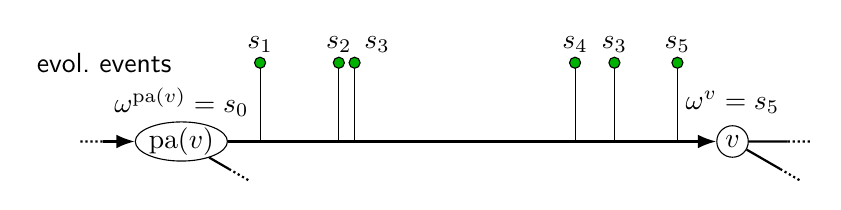
\begin{tikzpicture}[
%label position=0,
radius=2 pt,
treenode/.style={
ellipse,
draw,
minimum size=0.4 cm,
inner sep=0 pt,
}
]

% tree nodes
\node [treenode] at (0,0) (pa)
{\(\mathrm{pa}(v)\)};
\node [treenode] at (0:7 cm) (v)  {\(v\)};

\draw [thick, -Latex] (pa) -- (v);

% truncated edges
\draw[thick, solid]
(v) -- +(0:0.7 cm) coordinate(v1)
(v) -- +(-30:0.7 cm) coordinate(v2)
(pa) -- +(-30:0.7 cm) coordinate(w2)
;
\draw [thick, solid, -Latex] (180:1.0 cm) coordinate(pa2) -- (pa);
\draw[thick,densely dotted]
(v1) -- +(0:0.3 cm)
(v2) -- +(-30:0.3 cm)
(w2) -- +(-30:0.3 cm)
(pa2) -- ++(180:0.3 cm)
;

\path[align=right, anchor=east]
(pa) +(90:1) node {evol.~events}
;

\path
% substitutions
(1,1) coordinate(t1)
(2,1) coordinate(t5)
(2.2,1) coordinate(t6)
(5,1) coordinate(t8)
(5.5,1) coordinate(t13)
(6.3,1) coordinate(t14)
;

% plot
\draw plot[ycomb, mark=*, mark options={draw=black, fill=green!70!black}] coordinates{
% substitutions
(t1) (t5) (t6) (t8) (t13) (t14)
};


% labels for substitutions
\path[every node/.style={anchor=south}]
(t1) node {\(s_1\)}
(t5) node {\(s_2\)}
(t6) node[anchor=south west] {\(s_3\)}
(t8) node {\(s_4\)}
(t13) node {\(s_3\)}
(t14) node {\(s_5\)}
;

\path
(pa) +(90: 0.5 cm) node[anchor=center] {\(\omega^{\mathrm{pa}(v)}=s_0\)}
(v) +(90: 0.5 cm) node[anchor=center] {\(\omega^v=s_5\)}
;



\end{tikzpicture}
\end{document}


